\documentclass{article}
\usepackage{tikz}
\usepackage[x11names, rgb]{xcolor}

\begin{document}
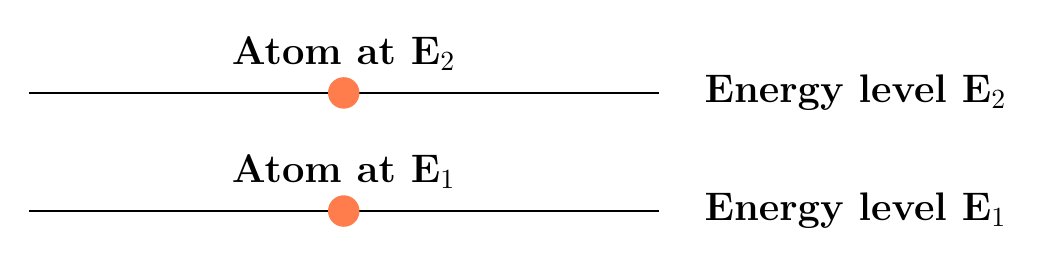
\begin{tikzpicture}

\definecolor{atom_red}{HTML}{FF4500}

\draw[thick] (0,3) -- (8,3);
\draw[thick] (0,1.5) -- (8,1.5);

\node at (10.5, 3) {\textbf{\Large Energy level E$_{2}$}};
\node at (10.5, 1.5) {\textbf{\Large Energy level E$_{1}$}};

\fill[atom_red!70] (4,3) circle (.2cm);
\fill[atom_red!70] (4,1.5) circle (.2cm);

% \node at (5, 0) {\textbf{\Huge Energy Level Diagram}};
% \node at (5, -1) {\textbf{\Huge of an Atom}};

\node at (4, 3.5) {\textbf{\Large Atom at E$_{2}$}};
\node at (4, 2) {\textbf{\Large Atom at E$_{1}$}};

\end{tikzpicture}
\end{document}
